A controller hardware in the loop (CHIL) simulation was setup to validate the algorithm in a real-time environment. 
The block layout of the CHIL simulation is shown in Fig. \ref{fig:RT_block}. The power system shown in Fig. \ref{fig:simulation_grid} is simulated in real time in a digital real-time simulator (DRTS) with a time step of 50 ${\mu}s$. This system is modeled for detailed electromagnetic transient simulation unlike the phasor simulation model used in the offline simulation. The A* based ESM algorithm is implemented in python 2.7 on a windows machine. The specifications of the machine is given in Table \ref{tab:PC}. The communication link between the DRTS and windows machine was established using TCP/IP. The DRTS sent the windows machine running the ESM the current PV generation ($P_{PV}(t)$), the current load ($P_load(t)$) and the current energy storage state of charge ($ES_{SOC}(t)$). The RTP, Load and PV prediction profiles are fed to the ESM by a pregenerated MATLAB formatted data (MAT) file. The current RTP is also provided by the MAT file. After receiving the current status and predicted profiles the ESM determines the power the ES should provide for the current time period ($P_{ES}(t)$) and sends it back to the DRTS. The maximum time needed by the ESM to calculate The actual CHIL setup is represented in Fig. \ref{fig:LAB_REAL}. 

\begin{table}[htb]
\caption{Windows machine specification}
\label{tab:PC}
\centering
\begin{tabular}{|l|l|}
\hline
Operating system & Windows 10 Home 64-bit      \\ \hline
Processor        & Intel(R) Core(TM) i5-7300HQ \\ \hline
Memory           & 8192 MB RAM                 \\ \hline
\end{tabular}
\end{table}

\begin{figure}[!ht]
    \centering
    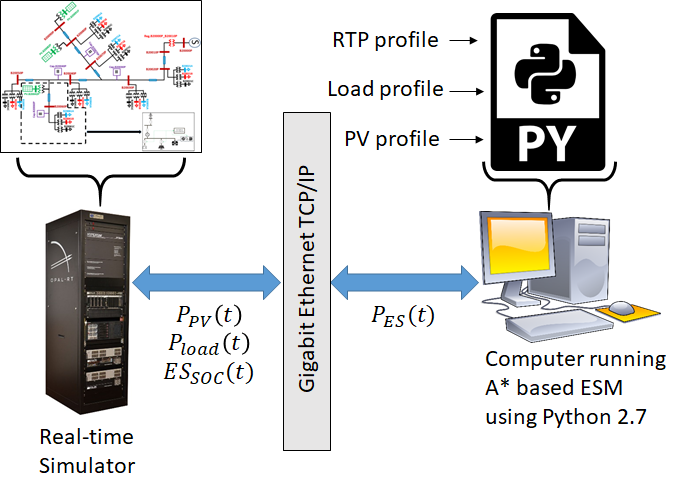
\includegraphics[width = \linewidth]{figs/RT_block.png}
    \caption{Block layout of CHIL}
    \label{fig:RT_block}
\end{figure}




\begin{figure}[!ht]
    \centering
    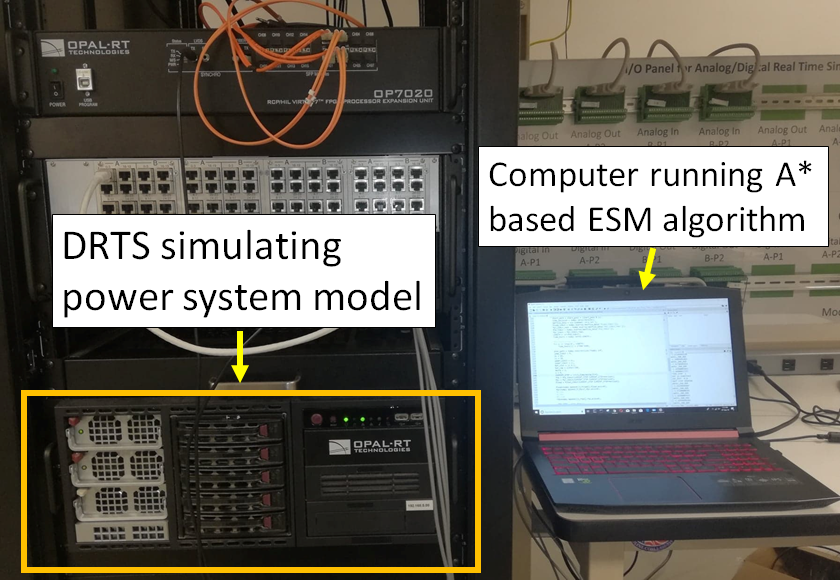
\includegraphics[width = \linewidth]{figs/LAB_REAL.png}
    \caption{Actual CHIL setup}
    \label{fig:LAB_REAL}
\end{figure}

For the CHIL simulation the ESM algorithm was set up according to the setup described in Section \ref{OFF}. The  SOC of the ESS is discretized in steps of 2\%, and the SOC is limited between  94\%  and  10\%. The time step and the control horizon chosen is 15 minutes. The ES is allowed to charge or discharge a maximum of 8\% of its total capacity during one time-step. The A* search runs every 15 minutes considering a 24 hours (96 time-steps) prediction horizon. The price profile used was the NYISO price profile. The different buying and selling price scenario with a sell back cost of 4 cents/kWh was considered. The cost of the ES was kept 12.3 cents/kWh. The simulation was run for 48 hours (192 time steps) in real-time. Fig. \ref{fig:RT_TESTING} shows the real-time and the offline simulation results for the 48 hours run. It can be seen that the real-time simulation result shown by the dotted lines follows the off-line simulation result shown by the solid line. The results are similar to the first two days of Fig. \ref{fig:VAR_10_12_4} as expected. The real time simulation result differ from the offline result because of discretization of the SOC. The SOC of the ES is discretized in steps 2\%. Anything in between the steps is converted to the next step before feeding it in the algorithm. So the value of 16.2\% SOC from time step 40 is actually converted to 18\% before feeding into ESM the algorithm. In case of the offline simulation the ES model used in the algorithm was exactly the same as the ES model used in the simulation. For the real-time simulation that was not the case. The ES model in the real-time simulation was modeled for detailed electromagnetic transient simulation and represented more accurate representation of a real battery. This means that when the algorithm determines a charging signal for the ES model in the real-time simulation it does not exactly reach the desired state. Also there is the delay for the ESM algorithm to calculate the next state and send it back to the real-time simulation. The maximum delay was observed to be 4 seconds. All of these factors are responsible for the difference in the real-time and offline results. The real-time cost savings of the algorithm is shown in table \ref{tab:rt_cost}. 



\begin{figure}[!ht]
    \centering
    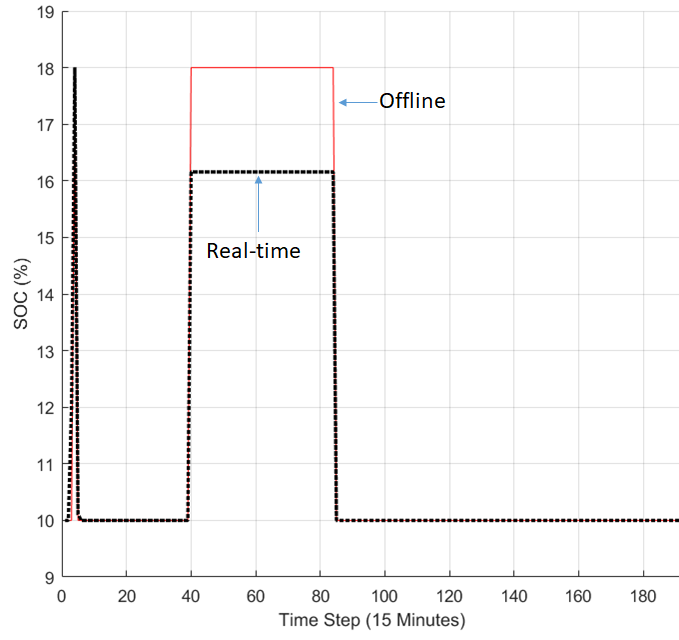
\includegraphics[width = \linewidth]{figs/RT_TESTING.png}
    \caption{Real-time vs offline result}
    \label{fig:RT_TESTING}
\end{figure}



\begin{table}[htb]
\centering
\caption{Real-time simulation cost (48 hours)}
\label{tab:rt_cost}
\begin{tabular}{|l|l|}
\hline
Case1               & \$1,662 \\ \hline
Case2                & \$1,823 \\ \hline
A* Case             & \$1,412 \\ \hline
A* savings (Case 1) & 15.04\% \\ \hline
A* savings (Case 2) & 22.55\% \\ \hline
\end{tabular}
\end{table}